\chapter[Paper: Supporting Wilderness Search and Rescue with Integrated Intelligence: Autonomy and Information at the Right Time and the Right Place]{Paper: Supporting Wilderness Search and Rescue with Integrated Intelligence: Autonomy and Information at the Right Time and the Right Place\footnote {Published in Twenty-Fourth AAAI 2010 (Association for the Advancement of Artificial Intelligence) conference. Authors are Lanny Lin, Michael Roscheck, Michael A. Goodrich, and Bryan S. Morse.}}
\label{chap:AAAI2010}

%=================================================================================
\begin{abstract}
%\begin{quote}
Current practice in Wilderness Search and Rescue (WiSAR) is analogous to an intelligent system designed to gather and analyze information to find missing persons in remote areas. The system consists of multiple parts --- various tools for information management (maps, GPS, etc) distributed across personnel with different skills and responsibilities. Introducing a camera-equipped mini-UAV into this task requires autonomy and information technology that itself is an integrated intelligent system to be used by a sub-team that must be integrated into the overall intelligent system. In this paper, we identify key elements of the integration challenges along two dimensions: (a) \textit{attributes of intelligent system} and (b) \textit{scale}, meaning individual or group. We then present component technology that offload or supplement many responsibilities to autonomous systems, and finally describe how autonomy and information are integrated into user interfaces to better support distributed search across time and space. The integrated system was demoed for Utah County Search and Rescue personnel. A real searcher flew the UAV after minimal training and successfully located the simulated missing person in a wilderness area.
%\end{quote}
\end{abstract}


%=================================================================================
\section{Introduction}
Wilderness Search and Rescue (WiSAR) can be thought of as an intelligent system designed to gather and analyze information to find and assist humans who are lost or injured in remote areas such as deserts and mountains. The system consists of multiple parts --- various tools for information management (maps, GPS, etc) distributed across personnel who have different skills. Using a camera-equipped mini-Unmanned Aerial Vehicle (UAV) to aid search can provide aerial imagery of a search area with the benefits of quick coverage of large areas, access of hard-to-reach areas, and lower cost than manned aircraft. 

Introducing a UAV into the WiSAR system requires autonomy and information technology that itself is an integrated intelligent system to be used by a WiSAR sub-team, and this sub-team and associated technology must be integrated into the overall intelligent system. This integration inevitably creates the need for new roles and responsibilities in order to manage the UAV and the aerial imagery~\cite{Adams2009Cognitive,Goodrich2007Using}. The task of creating a useful technology for supporting these roles is to make sure that these responsibilities are performed by appropriate people at an appropriate time with a satisfactory level of performance. Doing this requires the creation of algorithms that efficiently offload portions of responsibility to autonomous algorithms, creating an intelligent distributed system that facilitates the coordination and information management among roles. The need for efficiency creates the need to monitor and evaluate the performance of the system as a whole.

\begin{table}
\footnotesize
	\begin{center}
		\begin{tabular}{|p{3.4cm}|p{2cm}|p{4cm}|p{5cm}|}
			\hline
			 & \textbf{Capability} & \textbf{Information} & \textbf{Performance} \\
			 &  & \textbf{Management} & \textbf{Evaluation} \\
			 \hline
			 \rr \textbf{Intelligence of individual tools} & Autonomy & Flexibility & Progress toward individual goal \tn
			 \hline
			 \rr \textbf{Intelligence of distributed system} & Modularity & Fusion (Communication) & Collective progress/quality \tn
			\hline
		\end{tabular}
	\end{center}
\caption{Integration challenges defined along two dimensions. Horizontal dimension: attributes of intelligence. Vertical dimension: scale.}
\label{dimensions}
%\vspace*{-3ex}
\end{table}

In this paper we describe our efforts in developing autonomous algorithms and user interfaces that integrate components of machine and human intelligence with the goal of making UAV technology useful to real searchers in WiSAR. 
Thus, this paper is consistent with Drucker's definition of automation as a ``concept of the organization of work~\cite{Drucker2006Practice}.'' 
Intelligently organizing work requires that we identify key elements of the integration challenges organized along two dimensions: \textit{attributes of an intelligent system} (capability, information, performance evaluation) and \textit{scale} (individual versus group); see Table~\ref{dimensions}. We then present component algorithms  that augment or supplement search responsibilities. Next we describe how autonomy and information are integrated into user interfaces to better support distributed coordination of multiple searcher roles across time and space with respect to the integration challenges we identified.
%Then we use see-ability metrics to evaluate performances.

Validating an integrated system is always difficult. The goal of our research is to develop technology that provides help to real searchers; therefore, we believe a good way to validate our integrated system is to put it through a test in a real-world environment in front of real users. We summarize the experience of a recent field demo for Utah County Search and Rescue team representatives, where a real searcher acted as the UAV operator in a simulated search and rescue mission after minimal training.



%=================================================================================	
\section{Related Work}

The goal of our research is to support fielded missions in the spirit of Murphy's work~\cite{Casper2003Human}. UAV technology has emerged as a promising tool in supporting WiSAR~\cite{Bourgault2003Coordinated,Murphy2008Cooperative}. The UAV technology is an intelligent system with the integration of many component autonomous algorithms and user interfaces (related work for these components are referenced in their relative sections). Integration at this level requires tremendous effort. For example, building robots (GRACE and Spartacus) that are capable of attending a conference~\cite{Simmons2003Grace,Michaud2007Spartacus} required the integration of many technologies (e.g., localization/navigation, gesture/face recognition, and speech recognition/generation) and multiple modalities (e.g., mobility, vision, audition, and reasoning).

To integrate the UAV intelligent system into existing WiSAR practices --- which we argue is an intelligent system by itself~\cite{Setnicka1980Wilderness} --- creates additional challenges. Salas and Fiore~\shortcite{Salas2004Team} provide great insights on challenges across people and machines, and across time and space in distributed teams. Sycara and Lewis~\shortcite{Sycara2002Integrating} also asked the questions: 1) can a software agent perform the task? and 2) can the agent's assistance contribute toward team performance? Tso et al.\ ~\shortcite{Tso1999Multi} identified that integrating a UAV into the search task creates at least two roles: a pilot that controls the UAV and a sensor operator that analyzes the sensor outputs, and lessons from other search-related domains~\cite{Drury2003Awareness} show that multiple roles are required and these roles can be supported by autonomy algorithms and user interface technologies. These findings motivate and guide our research in developing UAV technology to support WiSAR operations.


\begin{figure}
\centering
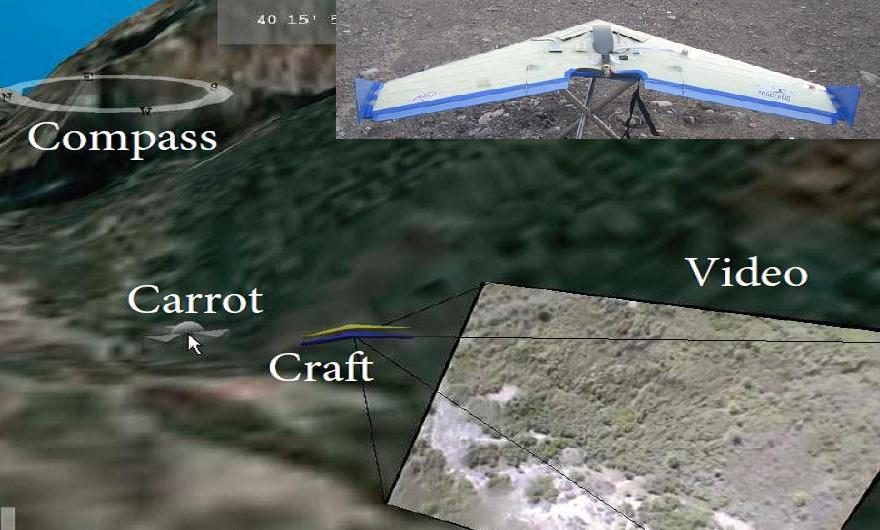
\includegraphics[width=6.0in]{UAVCarrot.jpg}
\caption{A screenshot of the UAV operator interface showing the position/orientation of the UAV, the orientation of the camera, and the projected video. (Top right: The UAV used in our research.)}
\label{UAVCarrot}
%\vspace*{-3ex}
\end{figure}


%=================================================================================	
\section{UAV Overview}

UAVs used in our research have wingspans of 42-50 inches, weigh approximately 2 lbs, and use lithium battery-powered propellers (see Figure~\ref{UAVCarrot}a). The airframes are designed so each UAV can stay aloft for up to two hours and travel at approximately 12-15 meters per second. The onboard sensors include three-axis rate gyroscopes, three-axis accelerometers, static and differential barometric pressure sensors, a GPS module, and a video camera on a gimbaled mount. An autopilot, designed by the BYU MAGICC lab~\cite{Beard2005Autonomous}, enables roll and pitch angle stabilization, attitude stabilization, altitude control, and waypoint following. The UAV uses a 900 MHz radio transceiver for data communication and an analog 2.4 GHz transmitter for video downlink. The typical operating height above ground is 60--100 meters so the UAV can avoid trees and slight terrain variations while still provide enough resolution so a human form can be discerned in the video~\cite{Goodrich2008Supporting}.

%=================================================================================	
\section{Integration Challenges}

We organize integration challenges along two dimensions: attributes (capability, information management, and performance evaluation) and scale (individual tool vs distributed system), as shown in Table~\ref{dimensions}. We assert that an intelligent system should display several attributes associated with intelligence across multiple scales. Capability pertains to the identification and development of specialized behaviors. Information management focuses on how information is presented, handled, and shared. Performance evaluation deals with monitoring the health of the system or progress toward the intended task goal. In this section we use this taxonomy to describe components of the UAV technology in the context of WiSAR. 

The individual tools were designed partly in response to a cognitive task analysis conducted on the WiSAR domain to inform the design of UAV technology~\cite{Adams2009Cognitive}.
 
The analysis identified four primary search tactics used in WiSAR: \textit{hasty search}, \textit{constrained search}, \textit{high priority search}, and \textit{exhaustive search}. Also, observations from several user studies~\cite{Cooper2008Towards} show that the best perspective (e.g., chase, north-up) for detecting and localizing a target depends on the type of search and the type of distribution (likely places to find the missing person). These findings suggest that multiple control modes, path planning methods, and perspectives are needed to support various search tactics and scenarios. These are examples of the capability for \textit{individual tools}. Since autonomous algorithms can replace or supplement searcher responsibilities, a wide range of capability is desired.

%Integrating a UAV into the search task creates at least two roles: a pilot that controls the UAV and a sensor operator that analyze the sensor outputs~\cite{tso1999multi}. The roles are really just groupings of responsibilities associated with intelligently using an airborne camera. The task of creating a useful technology for supporting these roles is to make sure that these responsibilities are performed by appropriate people at an appropriate time with a satisfactory level of performance. 
For the WiSAR system, the cognitive task analysis also identified two key WiSAR subsystems; information acquisition and information analysis. Combining this result with observations from past field trials, we see four roles emerge when a UAV is integrated into the search~\cite{Goodrich2008Supporting}. \textit{UAV operator}: responsible for guiding the UAV and the gimbaled camera to various locations and monitoring the UAV; \textit{video analyst}: responsible for scanning and analyzing imagery to detect potential clues; \textit{mission manager}: responsible for managing the search and prioritizing efforts based on information obtained; \textit{ground searcher}: (when supporting the UAV) responsible for investigating potential clues found in aerial imagery. Each role consists of a grouping of responsibilities. The task of creating useful technology for supporting these distributed roles is to make sure that these responsibilities are performed by appropriate people at an appropriate time with a satisfactory level of performance. Since people may take on (partial) responsibilities of other roles, the video analyst and the UAV operator might share responsibilities, these behaviors suggest that capabilities of individual systems should be modular to mix and match across roles. \textbf{Modularity} is a requirement for an intelligent distributed system -- it is the adaptable chunking of responsibility and capability.

\textbf{Flexibility}, in information management, is the ability to appropriately match capability to task according to the information available to the operator.
%For the HRI, this means that we have a usable interface that promotes situation awareness and allows a human to easily task autonomy.
The cognitive task analysis indicated that WiSAR search is an iterative process of gathering, analyzing evidence and planning for gathering more evidence, where probability refinement plays an important part during search. The analysis also identified that searches require considerable human judgment, especially as new evidence is collected. These findings suggest that tools and autonomy need to be flexible so they can be interrupted, temporarily aborted, and possibly resumed later. For example, if an object is spotted in the video, the UAV operator stops the current flight pattern and loiters around the Point Of Interest (POI) to gather more information. Once the UAV operator aborts the loiter mode, the UAV automatically resumes the previous flight pattern to continue to gather information.

For a distributed system, Information \textbf{Fusion} is an important element that efficiently combines and presents information from various sources to a user and also shares information among multiple users. For example, the user interface for the UAV operator includes the terrain map, an icon indicating the position and attitude of the UAV, an integrated video feed projected onto the terrain map showing the direction of the gimbaled camera, and various meters showing UAV status (e.g., speed, altitude, battery life); see Figure~\ref{UAVCarrot}. Another example is a video analyst helping to annotate clues in video imagery, and communicating the data to the mission manager who can update the search plan accordingly.

For each individual tool, the ability to evaluate the quality and the progress toward the individual goal can be useful and represents the importance of performance evaluation. A coverage map, for example, improves the UAV operator's situation awareness of how well an area has been covered. Morse et al.~\cite{Morse2010UAV} defined two see-ability metrics (described in the See-ability section). An \textit{instantaneous see-ability} evaluation helps the video analyst get a sense of the quality of a single frame of video. As for the distributed system, an overall, or group quality evaluation is more appropriate. A mission manager might want to know the \textit{collective see-ability} to understand how well the terrain is seen by all frames of video or combined coverage of the UAV and ground searchers.

In the following three sections we match components of our UAV system to the three attributes (columns) of our intelligent system taxonomy and show how they support various searcher roles at the right time and the right place.



%=================================================================================	
\section{Autonomy Components}

This section presents a wide breadth of \textbf{autonomy} components currently in place to support searcher roles and responsibilities. They map to the \textbf{Capability} column in our taxonomy (Table~\ref{dimensions}). The \textbf{modular} design allows mix and match of autonomy components to support the distributed system. Here we use the term ``low-level autonomy'' to describe components that only involve simple math calculations in contrast to the term ``advanced autonomy,'' where complex algorithms and interrelationships are required.

%==================================================
\subsection{Low-Level Autonomy}

%=============================
\subsubsection{Autopilot:} Pitch/roll/yaw and altitude stabilization, attitude controls, and waypoint following.
\subsubsection{Deploy and retrieve:} Two auto launch modes (take off to waypoint, spiral take off) and two auto land modes (rally land, deep stall).
\subsubsection{Gimbaled camera control:} A point can be set on the terrain map so the gimbaled camera constantly aims at the point independent of the UAV's flight path.
\subsubsection{Path planning:} Simple flight patterns include spiral, lawnmowing, and Zamboni.
\subsubsection{Safety:} If no waypoint is set or after reaching the end of set path, the UAV loiters around last waypoint. If the UAV loses communication with the base, it automatically returns to base and loiters.

\begin{figure}
\centering
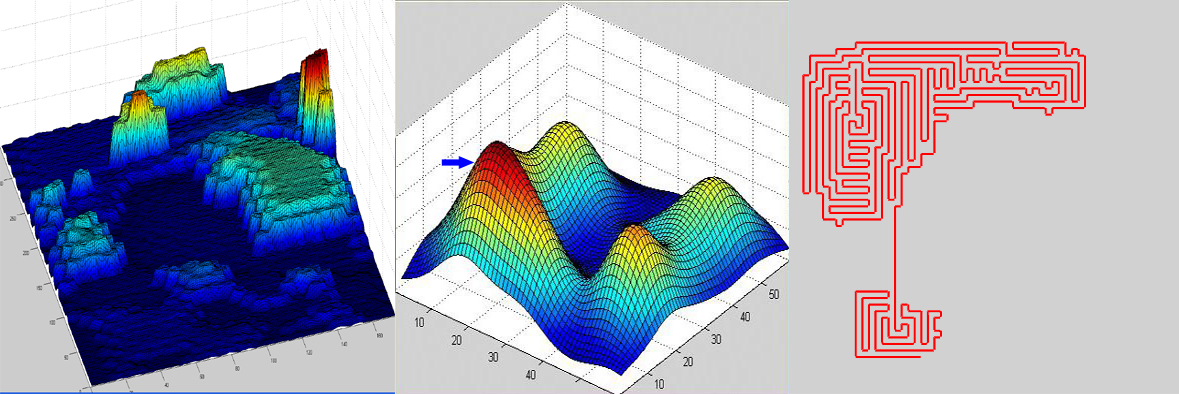
\includegraphics[width=6.0in]{maps.jpg}
\caption{Left: a posterior predictive distribution at 200th time step generated using the Bayesian model. Middle: a multimodal distribution used to test path planning (arrow marks starting point). Right: path generated using Intelligent Path Planning.}
\label{pathplanning}
%\vspace*{-3ex}
\end{figure}

%==================================================
\subsection{Advanced Autonomy}
%=============================
\subsubsection{Distribution Generation:}
A Bayesian model that incorporates past human behavior data and publicly available terrain data (topography, vegetation, and elevation) is used to automatically generate a posterior predictive distribution of the likely places of finding the missing person~\cite{Lin2009Bayesian}. The Markov chain Monte Carlo Metropolis-Hastings algorithm generates a temporal distribution showing how the distribution changes over time (Figure~\ref{pathplanning}). Given enough time, the distribution converges to a static state. The resulting distribution can be used by the search manager to prioritize search resources and develop search plans. It can also be used by the UAV operator for automatic path planning to maximize accumulated probability for a fixed flight duration.


%=============================
\subsubsection{Path planning:}
Two advanced path planning algorithms are described here: \textit{Generalized Contour Search}~\cite{Goodrich2008Supporting} and \textit{Intelligent Path Planning}~\cite{Lin2009UAV}. The ability to control the gimbaled camera to aim at a target point while orbiting enables a \textit{Generalized Contour Search} path planning algorithm. A queue of target points that follow the contours of the distribution of the missing person's likely locations can be created from which the algorithm interpolates (bicubic interpolation) and resamples at uniform distances. Lawnmower and spiral paths naturally emerge from the algorithm for uniform and Gaussian distributions respectively, and they are the optimal paths. It is also possible to use the algorithm to follow the contours of steep terrain by aiming the camera out the side of the UAV. The second path planning algorithm aims to maximize the accumulated probability for the path generated given a distribution, a starting point (optionally an ending point), and desired flight time. The camera footprint traverses a grid of probability nodes (enabled by the gimbaled camera) while the UAV approximates the path generated. Near optimal flight paths are generated using an evolutionary approach, where seed paths are generated using various hill-climbing and potential fields algorithms. Simulation results show the algorithm works well with a variety of probability distributions, including complicated multi-modal distributions (Figure~\ref{pathplanning}). These advanced algorithms enrich the autonomy tool set for the UAV operator and can potentially be useful for the \textit{high priority search} and \textit{exhaustive search} techniques when systematic coverage is desired.


%=============================
\subsubsection{Video mosaicing:}
The term \textit{mosaic} means to ``stitch'' together multiple frames of video of a static scene from a moving camera~\cite{Szeliski2006Image}. A real-time \textit{temporally local mosaic} technique~\cite{Morse2008Application} was developed using Harris corner detector to identify feature points and then using RANSAC~\cite{Fischler1981Random} to estimate the Euclidean transformation between each pair of frames. User studies using simulations and experience from field trials show that small mosaics of only the last few seconds of video is sufficient to provide both increased opportunity for detection and increased sense of relative spatial relationships. Figure~\ref{mosaic} shows an example of the local mosaic view where the same object is only visible in a few frames in original video but is visible for nearly one hundred frames using the technique.

\begin{figure}
\centering
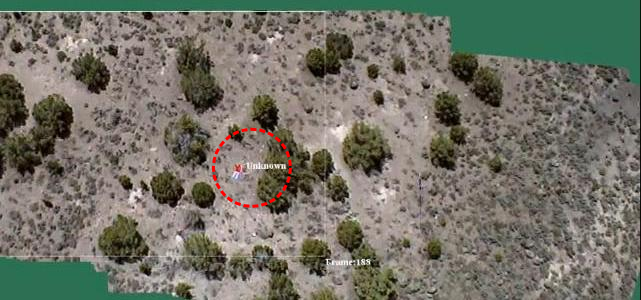
\includegraphics[width=6.0in]{mosaic.png}
\caption{Example of a video mosaic with an annotation (indicated by a red circle).}
\label{mosaic}
%\vspace*{-3ex}
\end{figure}


%=============================
\subsubsection{Anomaly detection (under development):}
A color anomaly detection algorithm is currently under development that adapts hyperspectral anomaly detection methods to find man-made objects in wilderness scenes. This algorithm adds another autonomy capability to the tool set and can recommend points of interest in the video imagery to the video analyst, potentially reducing mental workload. We mention this component in this paper for completeness.

%\begin{figure}
%\centering
%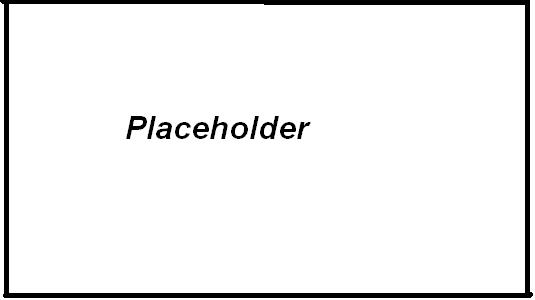
\includegraphics[width=3in]{Placeholder.jpg}
%\caption{Group of pictures showing GUI}
%\label{GUI}
%%\vspace*{-2ex}
%\end{figure}


%=================================================================================	
\section{User Interfaces}

In this section we describe the user interfaces developed to support various searcher roles with a focus on explaining how we integrate autonomy components (including control modes) and human intelligence. Interface techniques provides control \textbf{flexibility} with current information state, and information sharing and \textbf{fusion} improves the efficiency of the overall distributed system. They map to the \textbf{Information Management} column in our taxonomy (Table~\ref{dimensions}).

The UAV software consists of several components. \textbf{Phairwell} is the \textit{augmented virtuality} interface used to ``fly'' the UAV (see Figure~\ref{UAVCarrot}). The \textbf{Wonder Server} consists of central management software for capturing, storing, and retrieving video, UAV telemetry, annotations, and other related information. Finally, the \textbf{Wonder Client} is the GUI used by the video analyst and mission manager and provides video mosaic and annotation capabilities. Video and telemetry data are streamed from the Wonder Server.

%Control gimbaled camera separately from UAV path
%Various flying mode:
%- Manual 
%- Carrot and stick
%- Patterns
%- Contour following
%Break out of planned path and resume path afterwards


%=============================
%\vspace*{4 pt}
\noindent\textbf{Phairwell for UAV Operator:}
The UAV operator's main responsibilities include assigning the UAV a specific task, ensuring that it is properly performing that task while monitoring the UAV's ``health and safety,'' monitoring the live video, and interacting with the UAV when needed (e.g., once the video analyst spots a suspicious object, a change in the plan is made, or when the UAV needs attention). 

% Although the UAV has a high level of autonomy, another level of autonomy is used underneath Phairwell to manage things the UAV cannot. Since the UAV operator is provided with a vast range of autonomies, a high level of human intelligence is required to understand and select the right autonomies for each situation. In this section, we describe the different types of machine intelligence (autonomies) that are available to the operator.  

%HAG and automated altitude gain:
%It is important for the UAV to maintain a low, but safe, height above ground (HAG) so that objects in the video are large enough to be seen. However, the UAV is only aware of its current altitude and not the terrain around it. It would be a difficult and laborious task for the UAV operator to continually watch and adjust the UAV's altitude, especially with the rough terrain typical of WiSAR settings. This task is an ideal candidate for autonomy, completely freeing the operator of this responsibility. Phairwell continually monitors the geo-referenced terrain model simulation and looks forward in time along the UAVs flight path and instructs the UAV to adjust its altitude to maintain a consistent HAG.

%Flight modes and waypoints: 
Phairwell supports four flight modes while searching: \textit{manual}, \textit{carrot and camera}, \textit{flight plan}, and \textit{loiter now}. These modes represent autonomous behaviors that help the UAV operator efficiently assist the video analyst. \textit{Manual} mode commands the UAV to match a course and altitude set using the arrow keys. \textit{Carrot and camera} allows the operator to direct the UAV and camera with the mouse. \textit{Flight plan} mode commands the UAV to fly waypoints that the operator selects manually or that are generated automatically by one or more search patterns. The \textit{loiter now} mode interrupts the UAV's current behavior so the operator or UAV team can briefly ignore the UAV.

%Camera pointing: 
While directing the UAV is important, the primary goal is to manipulate the camera efficiently to provide the video analyst with the needed video. The speed of the UAV coupled with slow user response makes it impossible for the operator to manually track specific ground objects, a commonly required task. Instead, the UAV operator can select a terrain location in Phairwell and have the UAV fix the camera on the location. The UAV autonomy can maintain this lock, even when the UAV is turning rapidly or knocked about by gusts of wind. This allows the UAV operator to easily adjust the camera according to the needs of the video analyst.

%The ability to fix the camera on a specific location while loitering or flying around it is essential when investigating a point of interest (POI) or providing aerial support for ground searchers. When the terrain is sufficiently rough or the UAV is affected by wind, this camera pointing technique is also used to provide more stable and complete video coverage by briefly fixing the camera on discretized points along the flight path.

%Phairwell provides four perspective modes~\cite{goodrich2009lessons} (in addition to free-look) that automatically adjust the virtual camera to maintain the desired perspective. These are chase, track-up, north-up, and pilot perspectives. The ``best'' perspective depends on the task and the type of situation awareness the operator needs~\cite{cooper2008combine}. The chase perspective locks the virtual camera behind and above the UAV in order to provide visual information about the UAV's status and its local environment. The track-up and north-up perspectives both show the UAV from a satellite perspective where the UAV remains at the center of the screen. Track-up orients the map so that the UAV is always facing up while north-up fixes the map so north is always up. The pilot perspective shows provides a view from perspective of the UAV's camera. The operator must select the appropriate perspective mode based on their current task.

Although the UAV's autonomy allows it to fly a predefined flight plan, the UAV operator must often interrupt the autonomy and then resume it later. Phairwell allows the UAV operator to effortlessly change control modes, perform some task, and resume the previous control mode. This capability has been used routinely when the UAV is flying a search pattern and the video analyst sees something and wants the UAV to go back and take a closer look. This specific autonomy is described more fully in the next section.


%=============================
%\vspace*{4 pt}
\noindent\textbf{Wonder Client for Video Analyst:}
The Wonder Client interface serves as the video analyst's primary tool. They have the flexibility to select between either the live video or mosaiced views. The interface also provides tools to modify the brightness, contrast, and other image properties of the live video or mosaic, which often need to be adjusted to make objects more recognizable.

The video analyst also uses the Wonder Client to annotate the video. Annotations mark objects in the video with a timestamp and user notes so that they can be found quickly in the future. An example can be seen in Figure~\ref{mosaic}. When an annotation is placed on the video mosaic, it is tied to the geo-referenced coordinates of the underlying terrain. Therefore, annotations marked on previous video frames are automatically displayed on future frames, ensuring that the video analyst does not repeatedly identify the same object while also providing an efficient means of visually tracking the object. 

The video analyst can also indicate any geo-referenced location in the video as a POI that they want to immediately return to and investigate. The system then automatically communicates this information to Phairwell, giving the UAV operator the option of letting the autonomy redirect the UAV to investigate.


%=============================
%\vspace*{4 pt}
\noindent\textbf{Wonder Client for Mission Manager:}
The mission manager is responsible for assessing what has been searched and how well. This information is then used to plan further search efforts. While assessing ground searcher coverage is a common practice, UAV-assisted search adds a new and challenging aspect to this task. A coverage map showing the quality of the search is generated from the collective see-ability estimates to provide the mission manager with a complete view of the terrain the UAV video covered.

The Wonder Client gives the mission manager access to all the video analyst's POIs and annotations. The mission manager can then review the POIs and classify them as worth investigating or not. Those that are worth investigating are prioritized and placed in a pending search queue. The mission manager then assigns the UAV-team or ground searchers to investigate these points. Once the POI is located, the findings are reported back to the mission manager for assessment. However, investigations executed by the UAV-team will lead to this whole process being repeated.


%=============================
%\vspace*{4 pt}
\noindent\textbf{For Ground Searchers (under development):}
Successful search requires that ground searches quickly and thoroughly search their assigned area. We have begun development of a system that utilizes the concept of see-ability to support ground searchers in these efforts. A portable GPS device will be used to display a see-ability map, providing a visual representation of the thoroughness and quality of their search based on what they should have seen.

Communication between ground searchers and the UAV-team has proven limited and difficult. This same portable device will be used to bridge this communication gap. For example, when a ground searcher is assigned to investigate a POI, instead of radioing the GPS coordinates, the device will automatically receive the coordinates, overlay the UAV aerial imagery with the annotations, and provide the searcher with directions to the location.

%=============================
\section{See-ability Metrics}
\label{sec:seeability}
The ``see-ability'' metric~\cite{Morse2010UAV} was developed to address the challenge of understanding the search-related quality given by UAV video. This involves two different measures: \textit{instantaneous see-ability} measures the quality of a single video frame while \textit{collective see-ability} measures the overall quality provided by all video frames. They map directly to the \textbf{Performance Evaluation} column in our taxonomy (Table~\ref{dimensions}). 

The instantaneous see-ability computation uses the semi-accurate camera's location and pose information, terrain models, satellite imagery and computer vision techniques to geo-register each frame of video. The geo-registered frame is used to estimate the resolution with which each point in the video is seen. This metric could provide information about the quality of the video coverage for the video analyst. A user study showed that there was a moderately strong correlation between the instantaneous see-ability estimates and measured detection rates~\cite{Morse2010UAV}. Collective see-ability is determined by the number of times each point has been seen, from what distance, and from which and how many different angles. This is done by combining all of the instantaneous see-ability estimates available for a single point on the terrain. This metric provides the mission manager with information about the overall quality of the entire search.

%=================================================================================	
\section{Demonstration}

We believe a good way to validate our system is to demonstrate its usability in front of real searchers in a real-world environment. In the past several years, many field trials were operated by students pretending to be searchers. A demo to real searchers focuses more on the intended intelligence of the system. That led to a field demo on November 21, 2009 for representatives of the Utah County Search and Rescue team in a remote wilderness area in Elberta, Utah.

Three searchers participated in the demo. One searcher, R, acted as the UAV operator and flew the UAV in a simulated search and rescue mission while the other two searchers observed the mission and inquired about the capabilities of the system, the system structure, and the operation protocols. Professors and students of BYU volunteered as video analysts and ground searchers. R had received 30 minutes UAV operator training and also practiced in a simulated environment for a few hours. The mission objective was to locate a simulated missing person (a dummy placed in the wilderness) as quickly as possible in a team effort (UAV operator, video analyst, and ground searchers) utilizing the UAV technology. The responsibilities of the mission manager were split between the UAV operator and the video analyst. The missing person was successfully identified in the mosaic view, and the GPS location was radioed to the ground searchers, who successfully located the missing person. The entire mission completed in under 35 minutes.

The anomaly detection autonomy component and the GUI for ground searchers were not fully implemented and, therefore, were not included in the demo. Other than the distribution generation, intelligent path planning, and see-ability metric components (implemented and validated but not fully integrated), all other technologies described in this paper were available and functional.

We conducted an in-depth interview with R several weeks after the demo. Here we share only a portion of his feedback due to space limitations. R thinks the UAV operator interface is ``very easy to pick up'' and 30 minutes of training was plenty. His reason for practicing in the simulated environment was to explore and avoid silly mistakes. A few new features were available at the demo, but he was able to learn them quickly. He liked the video feed inside the UAV operator GUI because it helped him align the map with the video. One interesting incident was that he was able to identify the simulated missing person before the video analyst, probably the result of his trained eye. He also suggested that including ruler type tools in Phairwell could help him get a better perspective of the map. Feedback from his fellow searchers included comments such as ``That was cool!'' and ``This could work!''

Another key benefit of the demo is that it raises interest from the WiSAR community on technologies that can potentially assist WiSAR operations and opens the door for more direct collaboration between the WiSAR community and academic researchers in the near future.

%=================================================================================	
\section{Conclusions and Future Work}

To make UAV technology useful for WiSAR requires the integration of an intelligent UAV system into the existing intelligent WiSAR system. The autonomy components of the UAV technology also need to be integrated to support both individual searcher roles and the distributed system as a whole. We analyze and identify key elements of the integration challenges along two dimensions: attributes of intelligent system and scale. Component technologies are presented and matched to responsibilities of different searcher roles. Then we describe how components of autonomy are integrated into the user interfaces to support the integration of human intelligence for each search role in order to address the integration challenges we identified. Finally we validate the usefulness of the integrated system via a demonstration to Utah County Search and Rescue team representatives. A real searcher acted as the UAV operator and successfully located the simulated missing person using the intelligent UAV system through a team effort. Positive feedback from real searchers about the demonstration give us high hopes that research efforts in designing the UAV intelligent system can really help real WiSAR operations in the near future.

Immediate future work includes implementing and integrating system components identified in this paper but not included in the demo. Research is also planned for providing more flexibility for the existing tool set (e.g., interactive distribution modification and sliding autonomy for intelligent path planning). Long term goals focus on better integration of ground search situation awareness to improve system situation awareness and overall planning.